\documentclass[aspectratio=169,12pt,xcolor=table]{beamer}

% Modern theme
\usetheme{Madrid}
\usecolortheme{whale}

% Packages
\usepackage[utf8]{inputenc}
\usepackage[T1]{fontenc}
\usepackage{amsmath}
\usepackage{amsfonts}
\usepackage{amssymb}
\usepackage{graphicx}
\usepackage{booktabs}
\usepackage{tikz}
\usepackage{pgfplots}
\pgfplotsset{compat=1.18}
\usepackage{multicol}
\usepackage{adjustbox}
\usepackage{hyperref}

% Custom colors
\definecolor{niftyblue}{RGB}{0,71,171}
\definecolor{niftyorange}{RGB}{255,140,0}
\definecolor{niftygreen}{RGB}{34,139,34}
\definecolor{niftyred}{RGB}{220,20,60}
\definecolor{lightgray}{RGB}{240,240,240}

% Theme customization
\setbeamercolor{palette primary}{bg=niftyblue,fg=white}
\setbeamercolor{palette secondary}{bg=niftyorange,fg=white}
\setbeamercolor{palette tertiary}{bg=niftygreen,fg=white}
\setbeamercolor{palette quaternary}{bg=niftyblue,fg=white}
\setbeamercolor{structure}{fg=niftyblue}
\setbeamercolor{section in toc}{fg=niftyblue}
\setbeamercolor{subsection in toc}{fg=niftyorange}
\setbeamercolor{frametitle}{bg=niftyblue,fg=white}
\setbeamercolor{block title}{bg=niftyblue,fg=white}
\setbeamercolor{block body}{bg=lightgray,fg=black}

% Custom footer with full blue background
\setbeamertemplate{footline}{
  \leavevmode%
  \hbox{%
  \begin{beamercolorbox}[wd=.5\paperwidth,ht=2.5ex,dp=1ex,center,sep=0pt]{palette quaternary}%
    \usebeamerfont{title in head/foot}\insertshorttitle
  \end{beamercolorbox}%
  \begin{beamercolorbox}[wd=.5\paperwidth,ht=2.5ex,dp=1ex,right,sep=0pt]{palette quaternary}%
    \usebeamerfont{date in head/foot}\insertshortdate{}\hspace*{2em}
    \insertframenumber{} / \inserttotalframenumber\hspace*{2ex} 
  \end{beamercolorbox}}%
  \vskip0pt%
}

% Remove navigation symbols
\setbeamertemplate{navigation symbols}{}

% Hyperref setup to avoid errors
\hypersetup{
    pdfauthor={Anirudh Sharma, Anshul Choudhary, Gundra Rohan Reddy, Pushpdeep Singh Chandel, Rishabh Raj},
    pdftitle={Market Efficiency Through Information Theory},
    pdfsubject={Shannon Entropy Analysis of NIFTY Index},
    pdfkeywords={Shannon Entropy, Market Efficiency, NIFTY, Information Theory},
    colorlinks=true,
    linkcolor=niftyblue,
    urlcolor=niftyblue,
    citecolor=niftyblue
}

% Title information
\title[Shannon Entropy \& Market Efficiency]{\large Market Efficiency Through Information Theory}
\subtitle{\normalsize A Comparative Shannon Entropy Analysis of NIFTY Index vs. Top-10 Indian Large-Cap Stocks}

\author[Team]{
    \texorpdfstring{
        \begin{tabular}{c}
            \small Anirudh Sharma (22dcs002) \quad Anshul Choudhary (22dcs003) \\[0.1cm]
            \small Gundra Rohan Reddy (22dcs007) \quad Pushpdeep Singh Chandel (22dcs018) \\[0.1cm]
            \small Rishabh Raj (22dcs020)
        \end{tabular}
    }{Anirudh Sharma, Anshul Choudhary, Gundra Rohan Reddy, Pushpdeep Singh Chandel, Rishabh Raj}
}

\institute[NIT Hamirpur]{
    \small Department of Computer Science and Engineering \\
    National Institute of Technology Hamirpur
}
\date{} % Remove date from titlepage

\begin{document}

% ========================= SLIDE 1: TITLE =========================
\begin{frame}[plain]
\vspace{0.5cm}
\titlepage
\vspace{-1.2cm}
\begin{center}
    \textcolor{niftyorange}{\rule{0.8\textwidth}{2pt}}
    \vspace{0.1cm}
    
    {\small \textit{Information Theory and Coding}} \\
    \vspace{0.1cm}
    {\small \textit{Semester-7 (Batch: 2022-2027)}} \\
    \vspace{0.2cm}
    {\small October 28, 2025}
\end{center}
\end{frame}

% ========================= SLIDE 2: OUTLINE =========================
\begin{frame}[allowframebreaks]{Presentation Outline}
\tableofcontents[hideallsubsections]
\end{frame}

% ========================= SECTION 1: INTRODUCTION =========================
\section{Introduction}

\begin{frame}{Research Motivation}
\begin{columns}[T]
\begin{column}{0.5\textwidth}
    \textbf{Key Questions:}
    \begin{itemize}
        \item How efficient is the Indian stock market?
        \item Can information theory quantify market randomness?
        \item Is NIFTY more efficient than individual stocks?
    \end{itemize}
    
    \vspace{0.5cm}
    \textbf{Why Shannon Entropy?}
    \begin{itemize}
        \item Measures uncertainty and randomness
        \item Higher entropy = More unpredictable
        \item Aligns with Efficient Market Hypothesis
    \end{itemize}
\end{column}

\begin{column}{0.5\textwidth}
    \begin{block}{Research Hypothesis}
        \textcolor{niftyblue}{\textbf{Diversified indices exhibit higher Shannon entropy than individual stocks, indicating greater market efficiency.}}
    \end{block}
    
    \vspace{0.3cm}
    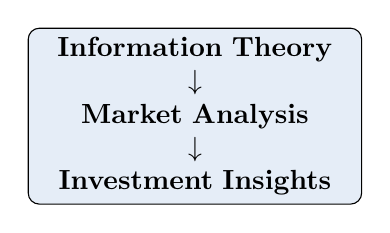
\begin{tikzpicture}
        \node[draw, fill=niftyblue!10, rounded corners, text width=4cm, align=center] at (0,0) {
            \textbf{Information Theory} \\
            $\downarrow$ \\
            \textbf{Market Analysis} \\
            $\downarrow$ \\
            \textbf{Investment Insights}
        };
    \end{tikzpicture}
\end{column}
\end{columns}
\end{frame}

\begin{frame}{Efficient Market Hypothesis (EMH)}
\begin{center}
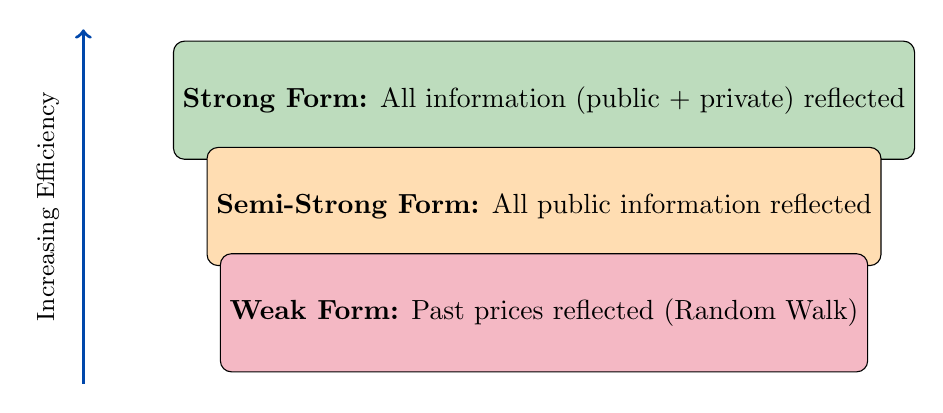
\begin{tikzpicture}[scale=0.9]
    % Three levels
    \node[draw, fill=niftygreen!30, rounded corners, minimum width=8cm, minimum height=1.5cm] at (0,3.5) {
        \textbf{Strong Form:} All information (public + private) reflected
    };
    \node[draw, fill=niftyorange!30, rounded corners, minimum width=8cm, minimum height=1.5cm] at (0,2) {
        \textbf{Semi-Strong Form:} All public information reflected
    };
    \node[draw, fill=niftyred!30, rounded corners, minimum width=8cm, minimum height=1.5cm] at (0,0.5) {
        \textbf{Weak Form:} Past prices reflected (Random Walk)
    };
    
    % Arrow
    \draw[->, very thick, niftyblue] (-6.5, -0.5) -- (-6.5, 4.5);
    \node[rotate=90] at (-7, 2) {\small Increasing Efficiency};
\end{tikzpicture}
\end{center}

\vspace{0.3cm}
\begin{block}{Entropy Connection}
Higher market efficiency $\rightarrow$ More random price movements $\rightarrow$ \textcolor{niftyblue}{\textbf{Higher Shannon Entropy}}
\end{block}
\end{frame}

% ========================= SECTION 2: METHODOLOGY =========================
\section{Methodology}

\begin{frame}{Shannon Entropy: Mathematical Foundation}
\begin{columns}[T]
\begin{column}{0.55\textwidth}
    \textbf{Shannon Entropy Formula:}
    \begin{equation*}
        \boxed{H(X) = -\sum_{i=1}^{n} p(x_i) \log_2 p(x_i)}
    \end{equation*}
    
    \vspace{0.1cm}
    \textbf{Where:}
    \begin{itemize}
        \item $H(X)$ = Shannon entropy (bits)
        \item $p(x_i)$ = Probability of outcome $i$
        \item $n$ = Number of possible outcomes
    \end{itemize}
    
    \vspace{0.2cm}
    \textbf{Interpretation:}
    \begin{itemize}
        \item $H = 0$ bits: Perfectly predictable
        \item $H = \log_2(n)$ bits: Maximum uncertainty
        \item Higher $H$: More information content
    \end{itemize}
\end{column}

\begin{column}{0.45\textwidth}
    \begin{block}{Example: Coin Flip}
        Fair coin: $p(H) = p(T) = 0.5$
        \begin{align*}
            H &= -0.5\log_2(0.5) \\
            &\quad - 0.5\log_2(0.5) \\
            &= 1.0 \text{ bit}
        \end{align*}
    \end{block}
    
    \vspace{0.2cm}
    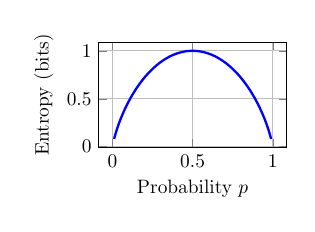
\begin{tikzpicture}[scale=0.7]
        \begin{axis}[
            xlabel={Probability $p$},
            ylabel={Entropy (bits)},
            domain=0.01:0.99,
            samples=100,
            grid=major,
            width=5cm,
            height=3.5cm
        ]
        \addplot[blue, very thick] {-x*ln(x)/ln(2) - (1-x)*ln(1-x)/ln(2)};
        \end{axis}
    \end{tikzpicture}
\end{column}
\end{columns}
\end{frame}

\begin{frame}{Research Design \& Data Collection}
\begin{columns}[T]
\begin{column}{0.5\textwidth}
    \textbf{Assets Analyzed (11 Total):}
    \begin{table}[h]
    \tiny
    \begin{tabular}{ll}
    \toprule
    \textbf{Asset} & \textbf{Ticker} \\
    \midrule
    \rowcolor{niftyblue!20} NIFTY Index & \textasciicircum{}NSEI \\
    Reliance Industries & RELIANCE.NS \\
    \rowcolor{lightgray} TCS & TCS.NS \\
    HDFC Bank & HDFCBANK.NS \\
    \rowcolor{lightgray} ICICI Bank & ICICIBANK.NS \\
    Bharti Airtel & BHARTIARTL.NS \\
    \rowcolor{lightgray} SBI & SBIN.NS \\
    LTIMindtree & LTIM.NS \\
    \rowcolor{lightgray} Infosys & INFY.NS \\
    HUL & HINDUNILVR.NS \\
    \rowcolor{lightgray} ITC & ITC.NS \\
    \bottomrule
    \end{tabular}
    \end{table}
\end{column}

\begin{column}{0.5\textwidth}
    \textbf{Data Specifications:}
    \begin{itemize}
        \item \textbf{Source:} Yahoo Finance (yfinance)
        \item \textbf{Period:} Jan 2019 - Sep 2025
        \item \textbf{Frequency:} Daily adjusted close
        \item \textbf{Observations:} $\sim$1,660 per asset
    \end{itemize}
    
    \vspace{0.1cm}
    \textbf{Analysis Pipeline:}
    \begin{enumerate}
        \item Download price data
        \item Compute log-returns: $r_t = \ln(P_t/P_{t-1})$
        \item Apply 90-day rolling window
        \item Calculate entropy using adaptive binning
        \item Statistical analysis \& visualization
    \end{enumerate}
\end{column}
\end{columns}
\end{frame}

\begin{frame}{Entropy Calculation Process}
\vspace{-0.1cm}
\begin{center}
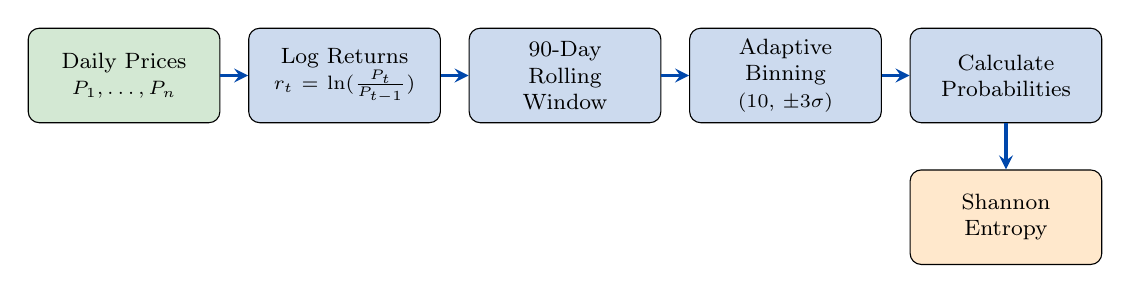
\begin{tikzpicture}[
    box/.style={rectangle, draw, fill=niftyblue!20, text width=2.2cm, align=center, rounded corners, minimum height=1.2cm, font=\footnotesize},
    arrow/.style={->, >=stealth, very thick, niftyblue}
]
    % Horizontal flow - 5 boxes in a row, then turn down
    \node[box, fill=niftygreen!20] (data) at (0,0) {Daily Prices \\ {\scriptsize $P_1, \ldots, P_n$}};
    \node[box] (returns) at (2.8,0) {Log Returns \\ {\scriptsize $r_t = \ln(\frac{P_t}{P_{t-1}})$}};
    \node[box] (window) at (5.6,0) {90-Day \\ Rolling \\ Window};
    \node[box] (bins) at (8.4,0) {Adaptive \\ Binning \\ {\scriptsize (10, $\pm 3\sigma$)}};
    \node[box] (prob) at (11.2,0) {Calculate \\ Probabilities};
    \node[box, fill=niftyorange!20] (entropy) at (11.2,-1.8) {Shannon \\ Entropy};
    
    % Arrows
    \draw[arrow] (data) -- (returns);
    \draw[arrow] (returns) -- (window);
    \draw[arrow] (window) -- (bins);
    \draw[arrow] (bins) -- (prob);
    \draw[arrow] (prob) -- (entropy);
\end{tikzpicture}
\end{center}

\vspace{0.3cm}
\begin{block}{Adaptive Binning Strategy}
\begin{itemize}
    \item Creates 10 bins within $\pm 3\sigma$ range of the data
    \item Captures data distribution more effectively than fixed binning
    \item Provides better discrimination between assets
\end{itemize}
\end{block}
\end{frame}

% ========================= SECTION 3: RESULTS =========================
\section{Key Results}

\begin{frame}{Primary Finding: Entropy Rankings}
\begin{center}
\textbf{\Large NIFTY Ranks 4th out of 11 Assets}
\end{center}

\vspace{0.1cm}
\begin{table}[h]
\centering
\small
\begin{tabular}{clcccc}
\toprule
\textbf{Rank} & \textbf{Asset} & \textbf{Mean} & \textbf{Std} & \textbf{CV(\%)} & \textbf{Note} \\
\midrule
1 & Bharti Airtel & 2.6607 & 0.0730 & 2.74 & Highest \\
2 & SBI & 2.6473 & 0.1378 & 5.21 & \\
3 & Reliance & 2.6408 & 0.1025 & 3.88 & \\
\rowcolor{niftyblue!30} \textbf{4} & \textbf{NIFTY} & \textbf{2.6368} & \textbf{0.1328} & \textbf{5.04} & \textbf{INDEX} \\
5 & TCS & 2.6343 & 0.0818 & 3.11 & \\
6 & ICICI Bank & 2.6294 & 0.0995 & 3.78 & \\
7 & LTIMindtree & 2.6177 & 0.1178 & 4.50 & \\
8 & HDFC Bank & 2.6114 & 0.1414 & 5.42 & \\
9 & ITC & 2.6073 & 0.1301 & 4.99 & \\
10 & HUL & 2.6054 & 0.1249 & 4.79 & \\
11 & Infosys & 2.5977 & 0.1507 & 5.80 & Lowest \\
\bottomrule
\end{tabular}
\end{table}

\begin{block}{Key Insight}
\textcolor{niftyblue}{\textbf{70\% of individual stocks show lower entropy than NIFTY}} \\
$\Rightarrow$ Index demonstrates higher randomness and market efficiency
\end{block}
\end{frame}

\begin{frame}{Visual Analysis: Comprehensive Results (Part 1)}
\vspace{0.2cm}
\begin{columns}[c]
\begin{column}{0.5\textwidth}
    \centering
    \includegraphics[width=\textwidth]{graphs/1.png}
    \vspace{0.1cm}
    
    {\small \textbf{Time Series Evolution}}
    
    {\footnotesize 90-day rolling Shannon entropy (2019-2025)}
\end{column}
\begin{column}{0.5\textwidth}
    \centering
    \includegraphics[width=\textwidth]{graphs/2.png}
    
    {\small \textbf{Distribution Comparison}}
    
    \vspace{-0.1cm}
    {\footnotesize Box plots across all assets}
\end{column}
\end{columns}
\end{frame}

\begin{frame}{Visual Analysis: Comprehensive Results (Part 2)}
\vspace{0.2cm}
\begin{columns}[c]
\begin{column}{0.5\textwidth}
    \centering
    \includegraphics[width=\textwidth]{graphs/3.png}
    
    {\small \textbf{Entropy-Volatility Relationship}}

    \vspace{-0.1cm}

    {\footnotesize Scatter plot analysis}
\end{column}
\begin{column}{0.5\textwidth}
    \centering
    \includegraphics[width=\textwidth]{graphs/4.png}
    \vspace{0.2cm}
    
    {\small \textbf{Statistical Summary}}
    
    {\footnotesize Comprehensive statistics table}
\end{column}
\end{columns}
\end{frame}

\begin{frame}{Entropy vs Volatility: The Efficiency Paradox}
\begin{columns}[T]
\begin{column}{0.5\textwidth}
    \textbf{Key Observation:}
    \begin{itemize}
        \item NIFTY: \textcolor{niftygreen}{\textbf{Low volatility}} (16.32\%)
        \item NIFTY: \textcolor{niftyblue}{\textbf{High entropy}} (2.6368 bits)
        \item Individual stocks: Higher volatility, lower entropy
    \end{itemize}
    
    \vspace{0.3cm}
    \begin{block}{Interpretation}
        \textbf{Efficiency Paradox:} \\
        Lower volatility $\neq$ Lower randomness \\
        \vspace{0.2cm}
        NIFTY's diversification creates:
        \begin{itemize}
            \item Stable price movements
            \item Unpredictable patterns
            \item Efficient information processing
        \end{itemize}
    \end{block}
\end{column}

\begin{column}{0.5\textwidth}
    \begin{center}
    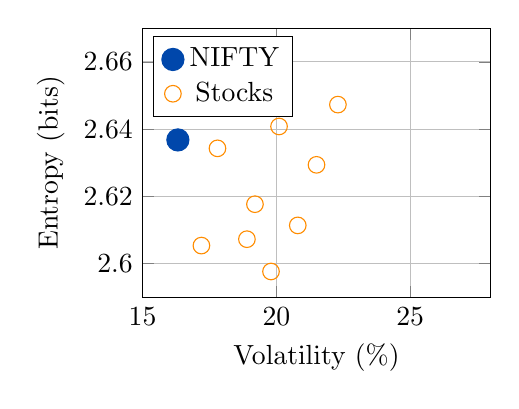
\begin{tikzpicture}
        \begin{axis}[
            xlabel={Volatility (\%)},
            ylabel={Entropy (bits)},
            width=6cm,
            height=5cm,
            grid=major,
            legend pos=north west,
            xmin=15, xmax=28,
            ymin=2.59, ymax=2.67
        ]
        % NIFTY point
        \addplot[only marks, mark=*, mark size=4pt, niftyblue] 
            coordinates {(16.32, 2.6368)};
        \addlegendentry{NIFTY}
        
        % Other stocks (approximate positions)
        \addplot[only marks, mark=o, mark size=3pt, niftyorange] 
            coordinates {
                (18.5, 2.6607) % Bharti
                (22.3, 2.6473) % SBI
                (20.1, 2.6408) % Reliance
                (17.8, 2.6343) % TCS
                (21.5, 2.6294) % ICICI
                (19.2, 2.6177) % LTIM
                (20.8, 2.6114) % HDFC
                (18.9, 2.6073) % ITC
                (17.2, 2.6054) % HUL
                (19.8, 2.5977) % Infosys
            };
        \addlegendentry{Stocks}
        \end{axis}
    \end{tikzpicture}
    \end{center}
    
    \vspace{0.2cm}
    \textcolor{niftyblue}{\textbf{NIFTY: Lowest volatility, 4th highest entropy}}
\end{column}
\end{columns}
\end{frame}

\begin{frame}{Temporal Patterns: Crisis Response}
\begin{columns}[T]
\begin{column}{0.5\textwidth}
    \textbf{COVID-19 Impact (March 2020):}
    \begin{itemize}
        \item Sharp entropy drop across all assets
        \item Increased market predictability
        \item Synchronized movements
    \end{itemize}
    
    \vspace{0.1cm}
    \textbf{Recovery Dynamics:}
    \begin{itemize}
        \item NIFTY: 3-4 months recovery
        \item Stocks: 6-8 months recovery
        \item Banking: Prolonged depression
    \end{itemize}
    
    \vspace{0.1cm}
    \textbf{Recent Period (2023-2025):}
    \begin{itemize}
        \item Entropy stabilization
        \item Return to pre-crisis levels
    \end{itemize}
\end{column}

\begin{column}{0.5\textwidth}
    \begin{center}
    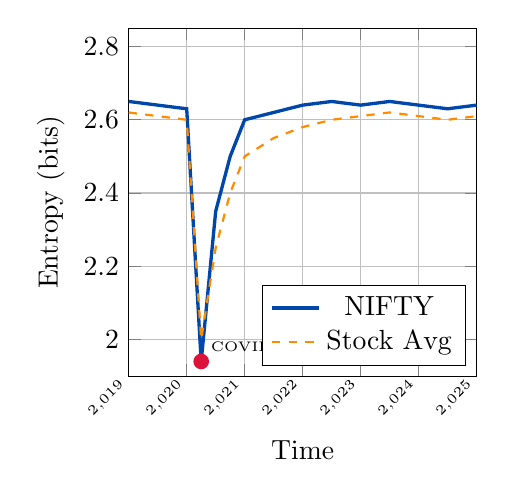
\begin{tikzpicture}
        \begin{axis}[
            width=6cm,
            height=6cm,
            xlabel={Time},
            ylabel={Entropy (bits)},
            xmin=2019, xmax=2025,
            ymin=1.9, ymax=2.85,
            xtick={2019, 2020, 2021, 2022, 2023, 2024, 2025},
            xticklabel style={font=\tiny, rotate=45, anchor=east},
            grid=major,
            legend pos=south east
        ]
        % NIFTY trend (stylized)
        \addplot[niftyblue, very thick] coordinates {
            (2019, 2.65) (2019.5, 2.64) (2020, 2.63)
            (2020.25, 1.94) (2020.5, 2.35) (2020.75, 2.50)
            (2021, 2.60) (2021.5, 2.62) (2022, 2.64)
            (2022.5, 2.65) (2023, 2.64) (2023.5, 2.65)
            (2024, 2.64) (2024.5, 2.63) (2025, 2.64)
        };
        \addlegendentry{NIFTY}
        
        % Stock average (stylized)
        \addplot[niftyorange, thick, dashed] coordinates {
            (2019, 2.62) (2019.5, 2.61) (2020, 2.60)
            (2020.25, 2.00) (2020.5, 2.25) (2020.75, 2.40)
            (2021, 2.50) (2021.5, 2.55) (2022, 2.58)
            (2022.5, 2.60) (2023, 2.61) (2023.5, 2.62)
            (2024, 2.61) (2024.5, 2.60) (2025, 2.61)
        };
        \addlegendentry{Stock Avg}
        
        % COVID marker
        \node[fill=niftyred, circle, inner sep=2pt] at (axis cs:2020.25,1.94) {};
        \node[above right] at (axis cs:2020.25,1.94) {\tiny COVID-19};
        \end{axis}
    \end{tikzpicture}
    \end{center}
\end{column}
\end{columns}
\end{frame}

\begin{frame}{Sectoral Analysis: High vs Low Entropy}
\begin{columns}[T]
\begin{column}{0.5\textwidth}
    \begin{block}{High Entropy Sectors}
        \textbf{1. Bharti Airtel (2.6607)} \\
        \small
        \begin{itemize}
            \item Regulatory uncertainties
            \item Technological disruption (5G)
            \item Competitive pressures
        \end{itemize}
        
        \vspace{0.2cm}
        \textbf{2. SBI (2.6473)} \\
        \small
        \begin{itemize}
            \item Economic cycle sensitivity
            \item Policy rate impacts
            \item NPL variations
        \end{itemize}
        
        \vspace{0.2cm}
        \textbf{3. Reliance (2.6408)} \\
        \small
        \begin{itemize}
            \item Diverse business exposure
            \item Oil price volatility
            \item Digital ventures uncertainty
        \end{itemize}
    \end{block}
\end{column}

\begin{column}{0.5\textwidth}
    \begin{block}{Low Entropy Sectors}
        \textbf{11. Infosys (2.5977)} \\
        \small
        \begin{itemize}
            \item Stable IT services model
            \item Predictable revenues
            \item Long-term contracts
        \end{itemize}
        
        \vspace{0.2cm}
        \textbf{10. HUL (2.6054)} \\
        \small
        \begin{itemize}
            \item Defensive FMCG characteristics
            \item Steady demand patterns
            \item Established brands
        \end{itemize}
        
        \vspace{0.2cm}
        \textbf{9. ITC (2.6073)} \\
        \small
        \begin{itemize}
            \item Strong market position
            \item Diversified product portfolio
            \item Predictable cash flows
        \end{itemize}
    \end{block}
\end{column}
\end{columns}

\vspace{0.3cm}
\begin{center}
\textcolor{niftyblue}{\textbf{Sector characteristics significantly influence entropy levels}}
\end{center}
\end{frame}

% ========================= SECTION 4: DISCUSSION =========================
\section{Discussion}

\begin{frame}{Market Efficiency Implications}
\begin{columns}[T]
\begin{column}{0.5\textwidth}
    \textbf{Evidence for EMH:}
    \begin{enumerate}
        \item \textcolor{niftygreen}{\textbf{Index Superiority}} \\
        NIFTY's high entropy (4th/11) supports diversification benefits
        
        \vspace{0.3cm}
        \item \textcolor{niftyblue}{\textbf{Information Aggregation}} \\
        Index aggregates cross-stock information $\rightarrow$ More unpredictable
        
        \vspace{0.3cm}
        \item \textcolor{niftyorange}{\textbf{Reduced Noise}} \\
        Individual stocks contain predictable company-specific patterns
    \end{enumerate}
\end{column}

\begin{column}{0.5\textwidth}
    \begin{center}
    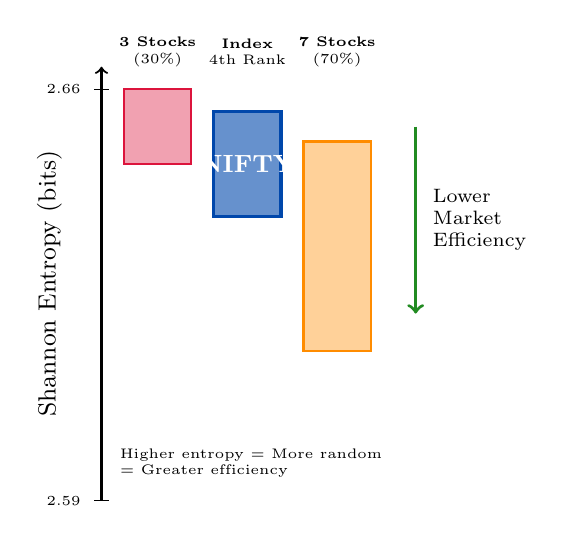
\begin{tikzpicture}[scale=0.95]
        % Bar chart style
        % Y-axis
        \draw[->, thick] (0,0) -- (0,5.8);
        \node[rotate=90, above, font=\small] at (-0.4,2.9) {Shannon Entropy (bits)};
        
        % Y-axis labels
        \draw (-0.1,0) -- (0.1,0) node[left, font=\tiny] at (-0.15,0) {2.59};
        \draw (-0.1,5.5) -- (0.1,5.5) node[left, font=\tiny] at (-0.15,5.5) {2.66};
        
        % Bars
        % Top 3 stocks (small, red)
        \fill[niftyred!40] (0.3,4.5) rectangle (1.2,5.5);
        \draw[niftyred, thick] (0.3,4.5) rectangle (1.2,5.5);
        \node[font=\tiny, align=center] at (0.75,6) {\textbf{3 Stocks}\\(30\%)};
        
        % NIFTY (medium, blue)
        \fill[niftyblue!60] (1.5,3.8) rectangle (2.4,5.2);
        \draw[niftyblue, very thick] (1.5,3.8) rectangle (2.4,5.2);
        \node[font=\small\bfseries, white] at (1.95,4.5) {NIFTY};
        \node[font=\tiny, align=center] at (1.95,6) {\textbf{Index}\\4th Rank};
        
        % Bottom 7 stocks (large, orange)
        \fill[niftyorange!40] (2.7,2.0) rectangle (3.6,4.8);
        \draw[niftyorange, thick] (2.7,2.0) rectangle (3.6,4.8);
        \node[font=\tiny, align=center] at (3.15,6) {\textbf{7 Stocks}\\(70\%)};
        
        % Efficiency arrow
        \draw[->, very thick, niftygreen] (4.2,5.0) -- (4.2,2.5);
        \node[right, font=\scriptsize, align=left] at (4.3,3.75) {Lower\\Market\\Efficiency};
        
        % Legend
        \node[font=\tiny, align=left] at (2,0.5) {Higher entropy = More random\\= Greater efficiency};
    \end{tikzpicture}
    \end{center}
    
    \vspace{0.1cm}
    \begin{alertblock}{Key Conclusion}
        \small
        \textbf{NIFTY outperforms 70\% of stocks} \\
        $\Rightarrow$ Index demonstrates superior efficiency
    \end{alertblock}
\end{column}
\end{columns}
\end{frame}

\begin{frame}{Practical Recommendations}
\begin{center}
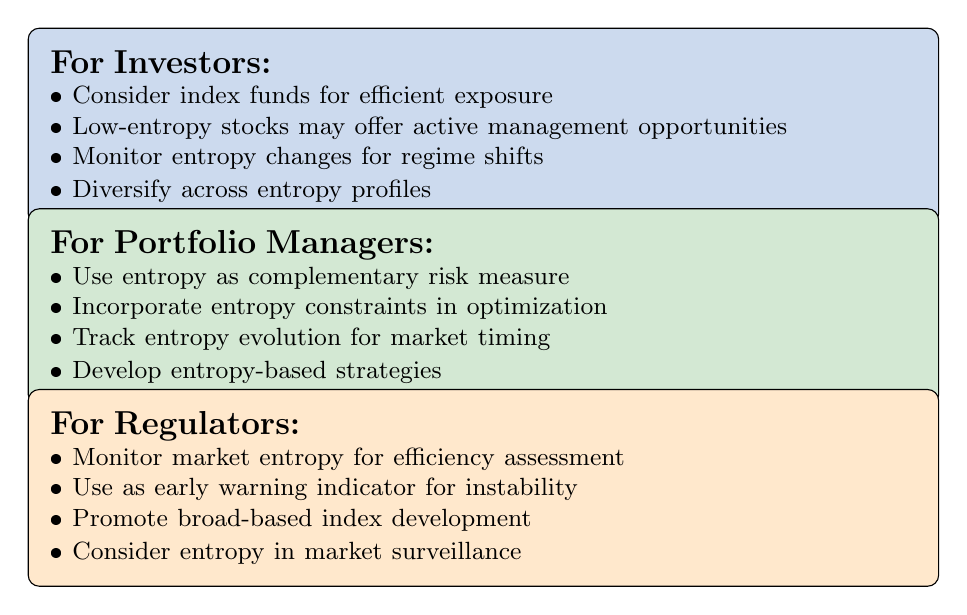
\begin{tikzpicture}[scale=0.85]
    % For Investors
    \node[draw, fill=niftyblue!20, rounded corners, text width=11cm, align=left, inner sep=8pt] at (0,5.5) {
        \textbf{\large For Investors:} \\
        \small
        • Consider index funds for efficient exposure \\
        • Low-entropy stocks may offer active management opportunities \\
        • Monitor entropy changes for regime shifts \\
        • Diversify across entropy profiles
    };
    
    % For Portfolio Managers
    \node[draw, fill=niftygreen!20, rounded corners, text width=11cm, align=left, inner sep=8pt] at (0,2.8) {
        \textbf{\large For Portfolio Managers:} \\
        \small
        • Use entropy as complementary risk measure \\
        • Incorporate entropy constraints in optimization \\
        • Track entropy evolution for market timing \\
        • Develop entropy-based strategies
    };
    
    % For Regulators
    \node[draw, fill=niftyorange!20, rounded corners, text width=11cm, align=left, inner sep=8pt] at (0,0.1) {
        \textbf{\large For Regulators:} \\
        \small
        • Monitor market entropy for efficiency assessment \\
        • Use as early warning indicator for instability \\
        • Promote broad-based index development \\
        • Consider entropy in market surveillance
    };
\end{tikzpicture}
\end{center}
\end{frame}

\begin{frame}{Comparison: Traditional vs Information-Theoretic Measures}
\begin{table}[h]
\centering
\small
\begin{tabular}{lcc}
\toprule
\textbf{Metric} & \textbf{Volatility-Based} & \textbf{Entropy-Based} \\
\midrule
\rowcolor{lightgray}
Focus & Risk/variance & Information/uncertainty \\
Interpretation & Dispersion & Randomness \\
\rowcolor{lightgray}
EMH connection & Indirect & Direct \\
Market efficiency & Not measured & Quantified \\
\rowcolor{lightgray}
Crisis detection & Price drops & Entropy drops \\
Predictability & Not captured & Core metric \\
\rowcolor{lightgray}
\textbf{Advantage} & \textbf{Well-established} & \textbf{Theoretical foundation} \\
\bottomrule
\end{tabular}
\end{table}

\vspace{0.3cm}
\begin{block}{Complementary Approach}
\begin{itemize}
    \item Volatility: Measures \textit{how much} prices move
    \item Entropy: Measures \textit{how random} movements are
    \item Together: Complete picture of market dynamics
\end{itemize}
\end{block}
\end{frame}

% ========================= SECTION 5: TECHNICAL DETAILS =========================
\section{Technical Implementation}

\begin{frame}[fragile]{Python Implementation Overview}
\begin{columns}[T]
\begin{column}{0.5\textwidth}
    \textbf{Key Components:}
    \begin{enumerate}
        \item \texttt{EntropyAnalyzer} class
        \item Data download module
        \item Rolling entropy calculator
        \item Visualization suite
        \item Statistical analysis engine
    \end{enumerate}
    
    \textbf{Libraries Used:}
    \begin{itemize}
        \item \texttt{yfinance} - Data collection
        \item \texttt{pandas} - Data manipulation
        \item \texttt{numpy} - Numerical computing
        \item \texttt{matplotlib} - Visualization
        \item \texttt{scipy} - Statistical tests
    \end{itemize}
\end{column}

\begin{column}{0.5\textwidth}
    \textbf{Entropy Calculation:}
    \begin{block}{}
        \tiny
        \texttt{def calculate\_entropy(data, \\
        \quad method='adaptive', n\_bins=10): \\
        \quad\quad \# Adaptive binning \\
        \quad\quad mean = np.mean(data) \\
        \quad\quad std = np.std(data) \\
        \quad\quad bins = np.linspace( \\
        \quad\quad\quad mean - 3*std, \\
        \quad\quad\quad mean + 3*std, \\
        \quad\quad\quad n\_bins + 1) \\
        \quad\quad hist, \_ = np.histogram(data, bins) \\
        \quad\quad prob = hist / hist.sum() \\
        \quad\quad entropy = -np.sum( \\
        \quad\quad\quad prob * np.log2(prob + 1e-10)) \\
        \quad\quad return entropy}
    \end{block}
    
    \vspace{0.2cm}
    \textbf{Total Implementation:} 450+ lines
\end{column}
\end{columns}
\end{frame}

\begin{frame}{Validation \& Robustness}
\begin{columns}[T]
\begin{column}{0.5\textwidth}
    \textbf{Statistical Validation:}
    \begin{itemize}
        \item Kolmogorov-Smirnov tests
        \item Significant differences (p < 0.01)
        \item 8 out of 10 comparisons significant
    \end{itemize}
    
    \vspace{0.3cm}
    \textbf{Robustness Checks:}
    \begin{enumerate}
        \item Multiple binning methods tested
        \item Window size sensitivity analysis
        \item Outlier treatment validation
        \item Cross-period consistency
    \end{enumerate}
\end{column}

\begin{column}{0.5\textwidth}
    \textbf{Binning Method Comparison:}
    \begin{table}[h]
    \tiny
    \begin{tabular}{lc}
    \toprule
    \textbf{Method} & \textbf{Discrimination} \\
    \midrule
    Equal-width & Poor \\
    Quantile (3 bins) & Very Poor \\
    Quantile (10 bins) & Moderate \\
    \rowcolor{niftygreen!20}
    \textbf{Adaptive} & \textbf{Best} \\
    \bottomrule
    \end{tabular}
    \end{table}
    
    \vspace{0.3cm}
    \begin{alertblock}{Best Practice}
        \small
        Adaptive binning with 10 bins based on $\pm 3\sigma$ range provides optimal entropy discrimination
    \end{alertblock}
\end{column}
\end{columns}
\end{frame}

% ========================= SECTION 6: CONCLUSIONS =========================
\section{Conclusions}

\begin{frame}{Research Findings Summary}
\begin{center}
\Large \textbf{Key Research Outcomes}
\end{center}

\vspace{0.1cm}
\begin{enumerate}
    \item \textcolor{niftyblue}{\textbf{Primary Finding:}} \\
    NIFTY exhibits higher entropy than 70\% of large-cap stocks (Rank: 4/11, Entropy: 2.6368 bits)
    
    \vspace{0.1cm}
    \item \textcolor{niftygreen}{\textbf{Efficiency Evidence:}} \\
    Index-level markets demonstrate characteristics consistent with EMH
    
    \vspace{0.1cm}
    \item \textcolor{niftyorange}{\textbf{Efficiency Paradox:}} \\
    NIFTY combines low volatility (16.32\%) with high entropy
    
    \vspace{0.1cm}
    \item \textcolor{niftyred}{\textbf{Crisis Response:}} \\
    NIFTY shows faster entropy recovery (3-4 months vs 6-8 months)
    
    \vspace{0.1cm}
    \item \textcolor{niftyblue}{\textbf{Sectoral Patterns:}} \\
    Clear entropy differences across sectors (Telecom highest, IT lowest)
\end{enumerate}
\end{frame}

\begin{frame}{Academic Contribution}
\begin{columns}[T]
\begin{column}{0.5\textwidth}
    \textbf{Theoretical Contributions:}
    \begin{itemize}
        \item Applied Shannon entropy to Indian markets
        \item Validated EMH through information theory
        \item Demonstrated index efficiency superiority
        \item Established entropy-volatility relationship
    \end{itemize}
    
    \vspace{0.3cm}
    \textbf{Methodological Innovations:}
    \begin{itemize}
        \item Adaptive binning strategy
        \item Rolling window entropy analysis
        \item Comprehensive visualization framework
        \item Integrated statistical validation
    \end{itemize}
\end{column}

\begin{column}{0.5\textwidth}
    \begin{block}{One-Line Summary}
        \textit{"70\% of large-cap stocks exhibit lower Shannon entropy than NIFTY, suggesting the index demonstrates higher randomness consistent with market efficiency theory."}
    \end{block}
    
    \vspace{0.3cm}
    \textbf{Publications Potential:}
    \begin{itemize}
        \item Information Theory applications
        \item Finance journals
        \item Market efficiency literature
        \item Emerging markets research
    \end{itemize}
\end{column}
\end{columns}
\end{frame}

\begin{frame}{Limitations \& Future Research}
\begin{columns}[T]
\begin{column}{0.5\textwidth}
    \textbf{Current Limitations:}
    \begin{enumerate}
        \item \textbf{Time Period:} \\
        2019-2025 (missing long history)
        
        \item \textbf{Binning Choice:} \\
        Methodology impacts results
        
        \item \textbf{Window Size:} \\
        90-day may miss some dynamics
        
        \item \textbf{Microstructure:} \\
        Intraday patterns not captured
        
        \item \textbf{Sample Size:} \\
        Limited to top 10 stocks
    \end{enumerate}
\end{column}

\begin{column}{0.5\textwidth}
    \textbf{Future Research Directions:}
    \begin{enumerate}
        \item \textcolor{niftyblue}{\textbf{Extended Analysis}} \\
        Longer historical periods
        
        \item \textcolor{niftygreen}{\textbf{Sector Studies}} \\
        Detailed industry analysis
        
        \item \textcolor{niftyorange}{\textbf{International}} \\
        Cross-country comparisons
        
        \item \textcolor{niftyred}{\textbf{High-Frequency}} \\
        Intraday entropy patterns
        
        \item \textcolor{niftyblue}{\textbf{Alternative Measures}} \\
        Rényi, approximate entropy
        
        \item \textcolor{niftygreen}{\textbf{Machine Learning}} \\
        Predictive entropy models
    \end{enumerate}
\end{column}
\end{columns}
\end{frame}

% ========================= CLOSING SLIDES =========================
\begin{frame}{References}
\small
\begin{enumerate}
    \item A. Shternshis, P. Mazzarisi, and S. Marmi, ``Measuring market efficiency: The Shannon entropy of high-frequency financial time series,'' \textit{Chaos, Solitons and Fractals}, vol. 162, 2022. \\
    \textcolor{niftyblue}{\url{https://doi.org/10.1016/j.chaos.2022.112403}}
    
    \vspace{0.1cm}
    \item H. Niu and Z. Hu, ``Information transmission and entropy-based network between Chinese stock market and commodity futures market,'' \textit{Resources Policy}, vol. 74, 2021. \\
    \textcolor{niftyblue}{\url{https://doi.org/10.1016/j.resourpol.2021.102294}}
    
    \vspace{0.1cm}
    \item J. F. Lavín, M. A. Valle, and N. S. Magner, ``Stock market pattern recognition using symbol entropy analysis,'' \textit{North American Journal of Economics and Finance}, vol. 73, 2024. \\
    \textcolor{niftyblue}{\url{https://doi.org/10.1016/j.najef.2024.102161}}
    
    \vspace{0.1cm}
    \item Project Repository: ``ITC-Entropy-Assignment'' \\
    \textcolor{niftyblue}{\url{https://github.com/anisharma07/ITC-Entropy-Assignment}}
\end{enumerate}
\end{frame}

\begin{frame}{Thank You!}
\begin{center}
{\Huge \textcolor{niftyblue}{\textbf{Questions?}}}

\vspace{1cm}
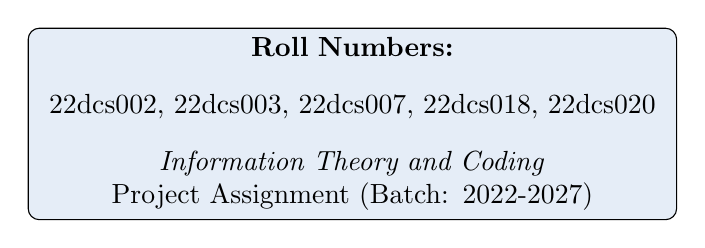
\begin{tikzpicture}
    \node[draw, fill=niftyblue!10, rounded corners, text width=8cm, align=center] {
        \textbf{Roll Numbers:} \\
        \vspace{0.3cm}
        22dcs002, 22dcs003, 22dcs007, 22dcs018, 22dcs020 \\
        \vspace{0.3cm}
        \textit{Information Theory and Coding} \\
        Project Assignment (Batch: 2022-2027)
    };
\end{tikzpicture}

\vspace{0.2cm}
\textcolor{niftyorange}{\rule{0.6\textwidth}{2pt}}

\vspace{0.2cm}
\textit{\small "Transforming financial chaos into quantifiable information through entropy"}
\end{center}
\end{frame}

\end{document}
